% ====================================================================
%+
% NAME:
%    multiperiodicvariables.tex
%
% CHAPTER:
%    variables.tex
%
% ELEVATOR PITCH:
%-
% ====================================================================

\section{Characterizing Multiperiodic, Short-Period Pulsating Variables}
\def\secname{multiperiodicvariables}\label{sec:\secname}

\credit{keatonb}

Most pulsating variable stars exhibit a superposition of multiple
simultaneous pulsation modes.  While these multiperiodic pulsators are
observationally more complex than classical pulsators, they communicate
a greater wealth of information about the stars.  Global nonradial
pulsations pass through and are affected by the interiors of stars, and
the measured frequencies of photometric variability are eigenfrequencies
of stars as physical systems.  Therefore, the observation and study of
photometric variability in multiperiodic pulsating stars is the most
powerful method by which we can probe stellar interiors.

The current state and modern tools of the field of asteroseismology are
thoroughly discussed by \citet{2010aste.book.....A}.  The locations of
the known classes of pulsating variable in the H-R Diagram are indicated
in their Figure 1.12, and a summary of their general
properties---including pulsation amplitudes and timescales---is provided
in their Appendix A.

Sections 8.6 and 8.7 of the Science Book express the anticipated
contributions that LSST will make to the study of pulsating variables.
While the sparseness of observations (low duty cycle) over the LSST
survey lifetime will make exact period solutions impossible for most
multiperiodic, short-period pulsating variables, the Science Book
correctly emphasizes that the photometric precision and multi-color
information will yield detections of variability that can be treated
statistically to determine the ensemble properties of different classes
of pulsating star.  The dependence of pulsational power on a star's
position in 5-color parameter space, as well as the relative pulsation
amplitudes in different passbands, informs the least understood aspects
of pulsation theory: mode selection and amplitude limiting mechanisms. A
thorough statistical view of pulsating stars requires on the order of
thousands of objects per type at a minimum, with robust detections of
variability in multiple passbands.

\subsection{The Case for ZZ Cetis}
\label{sec:\secname:targets}

Of the known classes of pulsating variable star, the ZZ Cetis
(pulsating hydrogen-atmosphere white dwarfs) are the faintest, and among
those with the lowest pulsation amplitudes.  These will be the most
difficult for LSST to detect and characterize, and they therefore
provide an important benchmark for assessing the effectiveness of
different proposed observing strategies for the study of pulsating
stars.  If LSST is well suited for ZZ Ceti science, it will be a useful
tool for all classes of pulsator.

Most details of ZZ Ceti stars are not strictly relevant to this
analysis, so we direct the interested reader to recent reviews by
\citet{2008ARA&A..46..157W}, \citet{2008PASP..120.1043F}, and
\citet{2010A&ARv..18..471A}.

As white dwarfs with atmospheres spectroscopically dominated by hydrogen
cool to between 12,500 and 10,600\,K, they are observed as the
photometrically variable ZZ Cetis.  The square root of the total
observed pulsational power (intrinsic root-mean-squared signal) in these
objects is on the order of 1\% and the mean pulsation periods are
$\sim$10\,min \citep{2006ApJ...640..956M}.  Because the pulsation
periods are $\ll$ the typical LSST revisit time, the survey will sample
the pulsations randomly in phase.

The ability to detect pulsations relies on the recognition that scatter
in the flux measurements significantly exceeds what can be attributed to
noise.  LSST's sensitivity to these pulsations depends on two things:
the photometric precision and the total number of measurements.  By
affecting these survey characteristics, the choice of observing strategy
impacts LSST's success in its goal of exploring the variable universe.
Strategies that maximize photometric precision and the total number of
visits in all filters optimize the survey toward this goal, but there are
tradeoffs between these dual requirements related primarily to exposure
time that are complicated and must be explored in MAF to be understood.

While consideration of observations across all filters together provides
the greatest sensitivity to detecting overall variability, the detection
of pulsational power in individual filters serves the science needs for
pulsating stars best.  Since LSST will not measure the specific periods
of complex, multi-periodic pulsating stars (at least not in the main
survey), LSST's potential to contribute significantly to this field lies
in the ability to measure relative pulsation power across many
passbands.  For ZZ Cetis in particular, there is a strong dependence of
the relative amplitudes measured in different filters on the geometry of
the pulsations---specifically the spherical degrees, $\ell$, of the
spherical harmonic wave patterns associated with the pulsation modes.
Determining the $\ell$ values associated with individual modes is
essential for comparing measured pulsation frequencies with those
calculated for asteroseismic stellar models.  The difficulty in
determining $\ell$ is currently the greatest limitation on white dwarf
asteroseismology. LSST has the potential to statistically constrain the
relative contributions of modes of different $\ell$ values to the
overall photometric variations.  The calculations by
\citet{1995ApJS...96..545B} of relative pulsation amplitudes in
different filters show that measuring the amplitude in the $u$ band is
essential for gaining leverage on this problem.

% --------------------------------------------------------------------

\subsection{Metrics}
\label{sec:\secname:metrics}

We have developed a custom MAF metric that calculates a ``variability
depth'' for every point on the sky equal to the magnitude limit for
detecting a population of photometric variables with a given
disk-integrated root-mean-squared (r.m.s.) underlying signal to a
desired level of completeness and a tolerable levels of contamination.
The metric makes the simplifying
assumptions that the typical revisit time for a field is longer than the
pulsation periods (appropriate for many pulsators, including ZZ Cetis),
and that the intrinsic variability takes the form of a Gaussian (which,
for multi-periodic pulsators, is supported by the central limit
theorem).  The metric relies on the total number of visits and
signal-to-noise per visit (scaled from the 5$\sigma$-depth, with
Gaussian errors assumed) for the calculation, and is included in {\tt
sims\_maf\_contrib} as {\tt VarDepth}.  Example output of this metric
is displayed in Figure~\ref{fig:vardepth}.

\begin{figure}
  \centering
  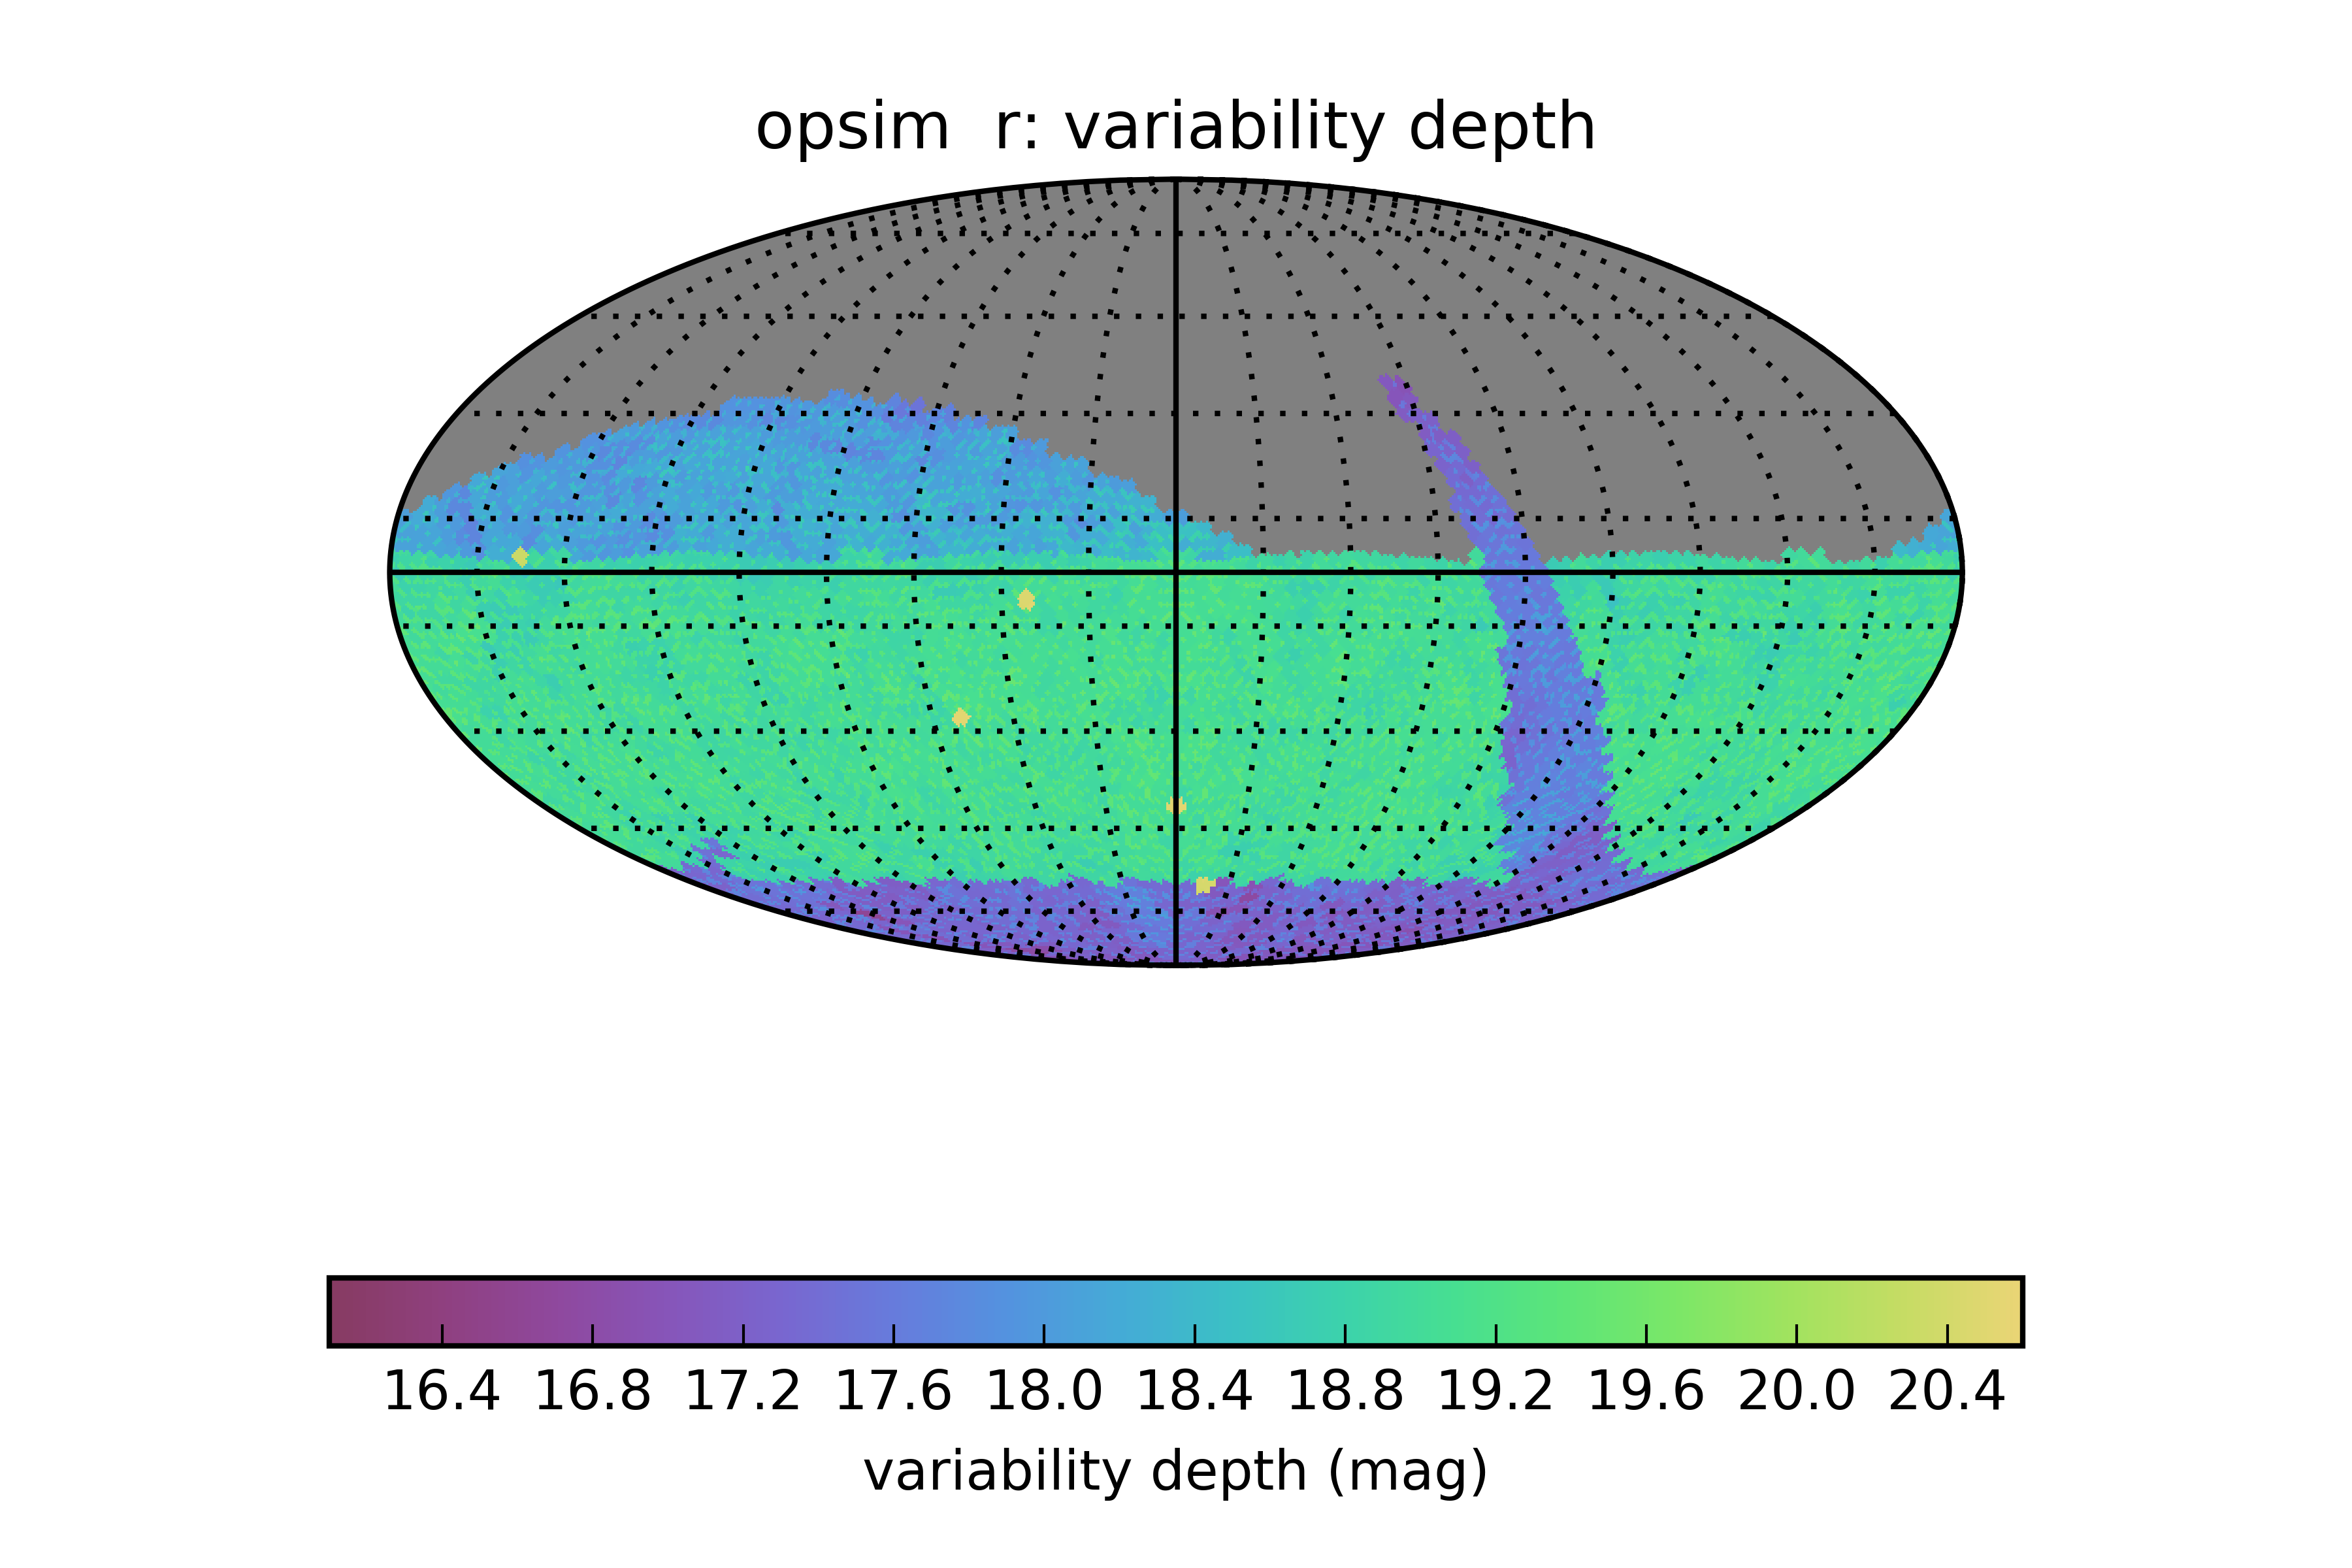
\includegraphics[width=0.76\columnwidth]{figs/vardepth.png}
  \caption{Example output of the {\tt VarDepth} MAF metric run on the
  current baseline cadence, {\tt minion\_1016}, after 10 years of survey
  operations. Input parameters and SQL queries were set to calculate the
  magnitude limit for detecting 90\% of pulsators with 1\% r.m.s.\
  variability from a cut on the measured variance in the $r$ band
  (allowing contamination from 10\% of nonvariable sources).}
  \label{fig:vardepth}
\end{figure}


We specialize this metric for the case of ZZ Ceti pulsators by including
maps of the expected distribution of ZZ Cetis in the Galaxy. These maps
were precomputed for the $u$ and $r$ filters by querying the CatSim
database for white dwarfs with an SQL constraint to include only those
with hydrogen atmospheres and with effective temperatures between 10,600
and 12,500 K (i.e., inside the ZZ Ceti instability strip).  While the
boundaries of the instability strip depend slightly on surface gravity,
the width of the strip does not change much, so these temperature cuts
yield representative counts.  The white dwarf spectral energy
distributions were calculated for CatSim by Pierre Bergeron et
al.\footnote{\url{http://www.astro.umontreal.ca/~bergeron/CoolingModels/}}\
The {\tt ZZCetiCounts} metric calculates the number of ZZ Cetis that we
expect to detect in each part of the sky, and the sum of the results
gives the total number of ZZ Cetis with variability detected by LSST.

The measured r.m.s.\ scatter from pulsations in ZZ Cetis is typically of
order $\sim$1\%, with a mean value around 3\%
\citep{2006ApJ...640..956M}.  Since we aim to statistically determine
the ensemble amplitude properties in multiple filters for a large
population of ZZ Cetis (particularly in the $u$ filter), we adopt the
following figure of merit for LSST's ability to study pulsating stars:
that significant variability should be detected in the $u$ band for at
least 1000 ZZ Cetis with r.m.s pulsational power of 1\% by the end of
the 10\,yr survey operations.  A sample of this size can be binned to track
changes in pulsational power as white dwarfs cool across the ZZ Ceti
instability strip, without the results being unduly influenced by random
sampling of inclination angle or the white dwarf mass distribution. It also
ensures that LSST contributes an order-of-magnitude improvement to the
number of ZZ Cetis known.

% --------------------------------------------------------------------

\subsection{OpSim Analysis}
\label{sec:\secname:analysis}

For comparison purposes, we calculate the number of ZZ Cetis detected in
both the $u$ and $r$ filters, assuming intrinsic r.m.s.\ variability of
1\% for two of the currently available OpSim runs: {\tt minion\_1016},
the current baseline cadence, and {\tt kraken\_1045}, with doubled
$u$-band exposure times. We require that 90\% of ZZ Cetis with 1\%
r.m.s.\  variability are detected to the computed ``variability depth,''
with a tolerance for up to 10\% of nonvariables with the same $u$ and
$r$ magnitudes to yield false detections.  The total number of ZZ Cetis
\emph{with this assumed r.m.s.\ variability level} detected for each of these
analyses is provided in Table~\ref{tab:zz1pertab}.


\begin{table}[h]
\begin{center}
    \caption{ZZ Ceti Recovery for 1\% R.M.S.\ Variability}\label{tab:zz1pertab}
    \begin{tabular}{| l | l | l |}
    \hline
    OpSim Run & Filter & \# ZZ Cetis \\ \hline
     {\tt minion\_1016} & $u$ & 9  \\
      & $r$ & 127 \\ \hline
    {\tt kraken\_1045}  & $u$ & 17\\
    & $r$ & 123  \\ \hline
    \end{tabular}
\end{center}
\end{table}

Clearly LSST appears to fall very short of the proposed figure of merit
by this measure.   The 1\% level of variability assumed for ZZ Cetis in
this treatment was chosen to ensure that the majority of lower-amplitude
ZZ Cetis are detected by LSST.  If we relax this constraint and repeat the
analysis with ZZ Cetis modeled as 3\% r.m.s.\ variables (the mean
r.m.s.\ variation observed), we get the results shown in Table~\ref{tab:zz3pertab}.
This approximates a total number of ZZ Cetis detected, allowing for
incompleteness to low amplitude.  While we still do not detect
$\sim$1000 ZZ Cetis in $u$, overall we see an increase in the total
number of detected ZZ Cetis by roughly an order of magnitude (in $r$),
with the {\tt kraken\_1045} simulation reaching markedly closer to the
$u$-band goal than the {\tt minion\_1016} strategy.


\begin{table}[h]
\begin{center}
    \caption{ZZ Ceti Recovery for 3\% R.M.S.\ Variability}\label{tab:zz3pertab}
    \begin{tabular}{| l | l | l |}
    \hline
    OpSim Run & Filter & \# ZZ Cetis \\ \hline
     {\tt minion\_1016} & $u$ & 197  \\
      & $r$ & 1601 \\ \hline
    {\tt kraken\_1045}  & $u$ & 325\\
    & $r$ & 1534  \\ \hline
    \end{tabular}
\end{center}
\end{table}


% --------------------------------------------------------------------

\subsection{Discussion}
\label{sec:\secname:discussion}

We emphasize again that ZZ Cetis make up the most difficult class of
pulsator to detect variability in, and that while other pulsators will
be better served by LSST, the currently proposed cadences capture a
less-than-complete census of pulsating variable stars.  More
sophistocated statistical techniques may come partially to the rescue
here as our MAF metric simply treats every star on a case-by-case basis,
rather than searching for increased scatter in a population of similar
stars.  Still, it appears that the science results for individual
low-amplitude ZZ Cetis will be severely limited.

The situation for higher amplitude ZZ Cetis and other types of variable
is better, and LSST observations of ZZ Cetis will certainly still be
worthy on careful analysis.  We note that the {\tt kraken\_1045}
strategy with 60\,s exposures in $u$ does a much better job of measuring
stellar variability overall, at the expence of a very minor decrease in $r$-band
detections.  We argue that any observing strategy that increases the number of
ZZ Cetis detected in the $u$ band will improve LSST's scientific yield for
\emph{all} stellar pulsation studies.

% ====================================================================
%
% \subsection{Conclusions}
%
% Here we answer the ten questions posed in
% \autoref{sec:intro:evaluation:caseConclusions}:
%
% \begin{description}
%
% \item[Q1:] {\it Does the science case place any constraints on the
% tradeoff between the sky coverage and coadded depth? For example, should
% the sky coverage be maximized (to $\sim$30,000 deg$^2$, as e.g., in
% Pan-STARRS) or the number of detected galaxies (the current baseline but
% with 18,000 deg$^2$)?}
%
% \item[A1:] ...
%
% \item[Q2:] {\it Does the science case place any constraints on the
% tradeoff between uniformity of sampling and frequency of  sampling? For
% example, a rolling cadence can provide enhanced sample rates over a part
% of the survey or the entire survey for a designated time at the cost of
% reduced sample rate the rest of the time (while maintaining the nominal
% total visit counts).}
%
% \item[A2:] ...
%
% \item[Q3:] {\it Does the science case place any constraints on the
% tradeoff between the single-visit depth and the number of visits
% (especially in the $u$-band where longer exposures would minimize the
% impact of the readout noise)?}
%
% \item[A3:] ...
%
% \item[Q4:] {\it Does the science case place any constraints on the
% Galactic plane coverage (spatial coverage, temporal sampling, visits per
% band)?}
%
% \item[A4:] ...
%
% \item[Q5:] {\it Does the science case place any constraints on the
% fraction of observing time allocated to each band?}
%
% \item[A5:] ...
%
% \item[Q6:] {\it Does the science case place any constraints on the
% cadence for deep drilling fields?}
%
% \item[A6:] ...
%
% \item[Q7:] {\it Assuming two visits per night, would the science case
% benefit if they are obtained in the same band or not?}
%
% \item[A7:] ...
%
% \item[Q8:] {\it Will the case science benefit from a special cadence
% prescription during commissioning or early in the survey, such as:
% acquiring a full 10-year count of visits for a small area (either in all
% the bands or in a  selected set); a greatly enhanced cadence for a small
% area?}
%
% \item[A8:] ...
%
% \item[Q9:] {\it Does the science case place any constraints on the
% sampling of observing conditions (e.g., seeing, dark sky, airmass),
% possibly as a function of band, etc.?}
%
% \item[A9:] ...
%
% \item[Q10:] {\it Does the case have science drivers that would require
% real-time exposure time optimization to obtain nearly constant
% single-visit limiting depth?}
%
% \item[A10:] ...
%
% \end{description}

% ====================================================================

\navigationbar
